\documentclass{standalone}

\usepackage{import}
\subimport{../../../}{preamble.tex}

\usepackage{pgfplots}

\begin{document}

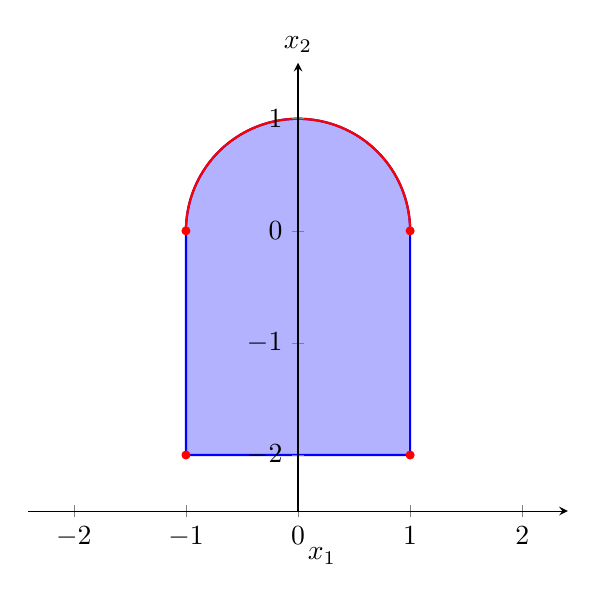
\begin{tikzpicture}
  \begin{axis}[
    axis on top,
    axis equal,
    axis x line=bottom,
    axis y line=center,
    xlabel={$x_1$},
    ylabel={$x_2$},
    xlabel style={right},
    ylabel style={above},
    xmin=-1.5,
    xmax=1.5,
    ymin=-2.5,
    ymax=1.5,
    ]

    \addplot[blue, fill=blue!30,  thick, domain=0:180, samples=500] ({cos(x)},{sin(x)}) -- (axis cs:-1, -2) -- (axis cs:1, -2) --cycle;

    \addplot[red,  thick, domain=0:180, samples=500] ({cos(x)},{sin(x)});
    
    \node[draw=red, fill=red, circle, inner sep=1] at (axis cs:-1, 0) {};
    \node[draw=red, fill=red, circle, inner sep=1] at (axis cs:1, 0) {};
    \node[draw=red, fill=red, circle, inner sep=1] at (axis cs:-1, -2) {};
    \node[draw=red, fill=red, circle, inner sep=1] at (axis cs:1, -2) {};
 \end{axis}
\end{tikzpicture}

\end{document}
